\documentclass[conference]{IEEEtran}

% Please include packages in the following file:
\input{packages.inc}

% Please define macros in the following file:
\input{macros-def.inc}

% Instructions for inserting comments:
%   \todo{t} for a TODO item
%   \modified{t} to mark as modified
% 	\nbb{t}{r} for inline region
%	\internalnote{t} for side-notes
%	\remarks{t} for inline comments in red
%	\del{t} for strikethrough
%	\ins{t} for suggestions
% ... read the input file for more
\input{comments.inc}

\begin{document}
\bstctlcite{MyBSTcontrol} % granular control for bib entries (cf. main.bib)

% The title
\title{Replication: Do Developers Discuss Design?}

% The authors
\author{
	\IEEEauthorblockN{Alvi Mahadi\IEEEauthorrefmark{1}, Neil Ernst\IEEEauthorrefmark{1}}
	\IEEEauthorblockA{\IEEEauthorrefmark{1}Department of Computer Science, University of Victoria, Victoria, Canada\\
		\{amahadi, nernst\}@uvic.ca}
}

% Configure here to get the paper title
\makeatletter
\hypersetup{
	pdftitle = {\@title},
	pdfsubject = {} % TODO e.g., SEAMS 2019
}
\makeatother

\maketitle

\begin{abstract}
% TODO
\end{abstract}

\begin{IEEEkeywords}
% TODO
\end{IEEEkeywords}

% contents
% !TEX root = main.tex
\section{Introduction}
\label{sect:introduction}

This is an example~\cite{marin-2017-what}.

% !TEX root = main.tex
\section{Related Work}
\label{sect:related_work}
To the best of our knowledge, this is the first replication work that takes the identical approach to replicate the work in~\cite{Brunet2014a}. However, this study has been revisited once before by~\cite{Shakiba2016} to determine if it is possible to predict a single commit message is about design or not. They manually annotated their own dataset that they used as train data and implemented a variety of classifiers to determine the best performing classifier. As they did not used the same dataset and procedures as~\cite{Brunet2014a}, they did not get the accuracy which was limited to 87.58\% for their best performing classifier, Random Forest.

If we do not limit ourselves to strict replication, we can find some literature which implements similar work. Maldonado in~\cite{Maldonado2017} tried to identify self admitted technical debt which can be perceived as one kind of design issue using Natural Language Processing. Like~\cite{Brunet2014a}, they manually classified a set of data which is used as training data for the Stanford Classifier, which is a Java implementation of a maximum entropy classifier. Using this classifier they achieved 90\% accuracy on test data and found out that, 23\% of the comment in both design and requirement comments are technical debt. A recent manual investigation on github discussion by Viviani~\cite{Viviani2018} shows some detailed information about the design discussions. He conducted an empirical study on the discussions and matched their result with~\cite{Brunet2014a} to validate their claim of 23-24\% design discussions being present in the discussions.   

% !TEX root = main.tex
\section{Data Set}
\label{sect:dataset}
The authors of the original paper took 90 projects that was present in the GHTorrent data set~\cite{Gousios2013} and discarded 13 projects due to having less than 50 discussions. In total they selected 77 projects with 102,122 discussions. Then out of the 77 projects, they randomly selected 5 projects. Then they randomly selected 200 discussions from each project, totaling 1,000 discussions for manual classification. Then the 1,000 discussions were manually classified by two individual authors of the paper. After the manual classification, 967 discussions were taken in which the classification by both authors matched. The 1000 discussions they took were randomly taken from five projects. Also they did not discuss or specify any rules for the manual classification of the 1,000 discussions. Due to the randomness of the data and the classification choice being very subjective, it is impossible to replicate the data they used. So we decided to contact them for their corpus of 1000 discussions and they provided us with the data. Also the 77 projects they took were not specified either. So we used their processed data from the GHTorrent database.

\noindent\textbf{discussions.csv}--- contains the 967 sentences that are manually classified by two of the authors of the paper, 226 (23\%) of these refer to `design' points and 741 (77\%) of them are other issues labeled as `general'. A sample of the file is shown in Table~\ref{tbl:discussions.csv}
\begin{table*}
	\centering
	\caption{Data sample in discussions.csv}
	\label{tbl:discussions.csv}
	\begin{tabular}{lccc} 
		\toprule
		\textbf{Discussion Text} & \textbf{Label}  \\
		\midrule
		Did you send a bug report comment upstream or something because otherwise we are gonna have to fix this again with the next version of assimp & general \\
		SSL contexts shouldnt be reused across connections see So its probably more appropriate to pass in factories directly & design \\
		\bottomrule
	\end{tabular}
\end{table*}

\noindent\textbf{rq\_1.csv}--- is a data file with 5,86,839 lines of data. Each line represents three columns separated by a space. The first column points to the repository and project name separated by `/'. The second column provides information about whether this discussion comes from an issue, commit or pull request with the associated commit, issue or pull request number. The third column represents the label that the classifier assigned. Table~\ref{tbl:rq_1.data} shows a sample of the data that this file contains.
\begin{table*}
	\centering
	\caption{Data sample in rq\_1.data}
	\label{tbl:rq_1.data}
	\begin{tabular}{lccc} 
		\toprule
		\textbf{Repository/Project} & \textbf{Event Category with Number}  & \textbf{Label}  \\
		\midrule
		akka/akka & akka/akka-commit\_comments-d9e0088f3cc537ea342f6fc4e99ee5319dfc94ae & general \\
		akka/akka & akka/akka-commit\_comments-3ce3f270dfce5da7aa5b6270b0559e2c3c0fff6f & design \\
		ariya/phantomjs & ariya/phantomjs-issue\_comments-10045 & design \\
		antirez/redis & antirez/redis-issue\_comments-160 & general \\
		\bottomrule
	\end{tabular}
\end{table*}

\noindent\textbf{rq\_2\_a.data}--- also contains 5,86,839 lines of data divided into four columns by single space that represents username of the contributor, commit/issue/pull request with respective number, label of the discussion and repository name/project name respectively as shown by the sample in Table~\ref{tbl:rq_2_a.data}.
\begin{table*}
	\centering
	\caption{Data sample in rq\_2\_a.data}
	\label{tbl:rq_2_a.data}
	\begin{tabular}{lccc} 
		\toprule
		\textbf{Username} & \textbf{Event Category with Number}  & \textbf{Label} & \textbf{Repository/Project}  \\
		\midrule
		viktorklang & akka/akka-commit\_comments-d9e0088f3cc537ea342f6fc4e99ee5319dfc94ae & general & akka/akka \\
		jboner & akka/akka-commit\_comments-a3026b3316dc5b34c3d37ce6fc56cc44bac1d561 & design & akka/akka \\
		antirez & antirez/redis-issue\_comments-646 & general & antirez/redis \\
		patriknw & akka/akka-pull\_request\_comments-149 & general & akka/akka \\
		\bottomrule
	\end{tabular}
\end{table*}

\noindent\textbf{rq\_2\_b.data}--- is a narrowed copy of `rq\_2\_a.data' that contains the username of the contributor, repository/project name and commit, issue or pull\_request with number that points to only the design label.

\noindent\textbf{rq\_2\_a\_c.data}--- hold 23,293 lines of data that is divided into three columns. The first column represents the repository name/project name, the second column shows the user name of the contributor. The last column points to the number of design discussions the user in the previous column addressed in the project defined by the first column. Table~\ref{tbl:rq_2_a_c.data} shows the sample of data in the file.  
\begin{table*}
	\centering
	\caption{Data sample in rq\_2\_a\_c.data}
	\label{tbl:rq_2_a_c.data}
	\begin{tabular}{lccc} 
		\toprule
		\textbf{Repository/Project} & \textbf{Username} & \textbf{Involvement in design discussions}   \\
		\midrule
		zurb/foundation & stewarty & 1 \\
		rails/rails & hassox & 1 \\
		rails/rails & stjhimy & 1 \\
		twitter/finagle & kolbasov & 1 \\
		cakephp/cakephp & atkrad & 1 \\
		zendframework/zf2 & ravids & 1 \\
		symfony/symfony & jdhoek & 6 \\
		joyent/node & paulfryzel & 1 \\
		mxcl/homebrew & hackdefendr & 9 \\
		\bottomrule
	\end{tabular}
\end{table*}

   
% !TEX root = main.tex 
\section{Replication}
\label{sect:replication}
We strictly followed the steps demonstrated in the paper. While replicating, we took the following steps:

\subsection{Stopwords Removal}
Stopwords are words that have the similar likelihood of occurring in documents regardless of the relevance of the query~\cite{Wilbur1992}. It is very important to remove stopwords to improve the performance of the classifier as well as reducing the size of the dataset. We have used the The \emph{Natural Language Toolkit's (NLTK)}\footnote{NLTK, https://www.nltk.org/}~\cite{Loper2002} english stopwords set to primarily remove some general stopwords. Then we have looked for some document specific stopwords ex. `lgtm' which is short form of `looks good to me' and removed them. The before and after status of a sentence for stopwords removal can be seen in Table~\ref{tbl:stopwords_removal}
  \begin{table}
  	\caption{Sample of sentence status before and after stopwords removal. The sentence on the top is the actual sentence. The bottom one is after removing the stopwords  }
  	\begin{tabular}{ p{3.25in}}
	 	\toprule
	  		Did you send a bug report comment upstream or something because otherwise we are gonna have to fix this again with the next version of assimp \\
  		\midrule
	  		send bug report comment upstream something otherwise gonna fix next version assimp \\
  		\bottomrule

  	\end{tabular}
  	\label{tbl:stopwords_removal}
  \end{table}   

\subsection{Feature Selection}  
\emph{Feature selection} is the process of selecting a subset of the terms occurring in the training set and using only this subset as features in text classification\footnote{https://nlp.stanford.edu/IR-book/html/htmledition/feature-selection-1.html}. Feature selection are used mainly for twos reason. \noindent\textbf{One}, it reduces the size of the effective vocabulary which is helpful to speed up the training for an expensive classifier like Decision Tree. \noindent\textbf{Two}, it often increases the accuracy by reducing the amount of noisy feature in a corpus. In the original paper, they combined two methods of feature extraction. \noindent\textbf{First}, they have found and ranked the bigram\footnote{https://en.wikipedia.org/wiki/Bigram} collection of other association measures by first constructing it for all bigrams in a given sequence. Then they have provided the Pearson's chi-square as the score to return the top bigrams. \noindent\textbf{Second}, they have counted every bigram by iterating through every word in the sentence to find out the pair and assigned a true/false value for them. Table~\ref{tbl:feature_selection} shows the dictionary after implementing combined bigram features.
  \begin{table}
	\caption{Sample of the dictionary of words that is returned after using combined bigram features. In the top: the original text after stopwords removal. In the bottom: The dictionary of combined word bigrams}
	\begin{tabular}{ p{3.25in}}
		\toprule
		martijnvg seems reasonable done \\
		\midrule
		{`martijnvg': True, `seems': True, `reasonable': True, `done': True, (`martijnvg', `seems'): True, (`reasonable', `done'): True, (`seems', `reasonable'): True} \\
		\bottomrule
		
	\end{tabular}
	\label{tbl:feature_selection}
\end{table}

\subsection{Classification and Validation}
We have used Naive Bayes and Decision Tree classifier as the classification models for the sentences like they did in the paper. Also following them, we have also used 10-fold cross validation method to validate the performance of the classifiers. We have divided the whole dataset in 10 chunks containing almost 100 sentences in each chunk. Then we have taken 9 chunks to train our model and then tested it with the other chunk we left untouched. We repeated this procedure for 9 more times each time moving onto the next chunk to use it as test and the rest of them as train. We are calculating the accuracy of every pass which is essentially the fraction of corresponding values that are equal to the test label. Finally, we have calculated the mean of 10 passes to estimate the overall accuracy for each classifier. We have also estimated the performance of each classifier in terms of time. To do that, we have taken into account the difference between the start time of the classification and the end time. This can demonstrate the cost of each classifier in time.

\subsection{Information Extraction}
Due to the lack of clarification in the paper about which 77 projects were used and due to the randomness in choice of the 1,02,122 discussions that were taken from the 77 projects, we used the pre-processed dataset from~\cite{Brunet2014a} to extract the information needed for answering the research questions. We used a quantitative approach to extract different information from the \emph{.data} files. 
% !TEX root = main.tex
\begin{figure}[hbt]
	\centering
	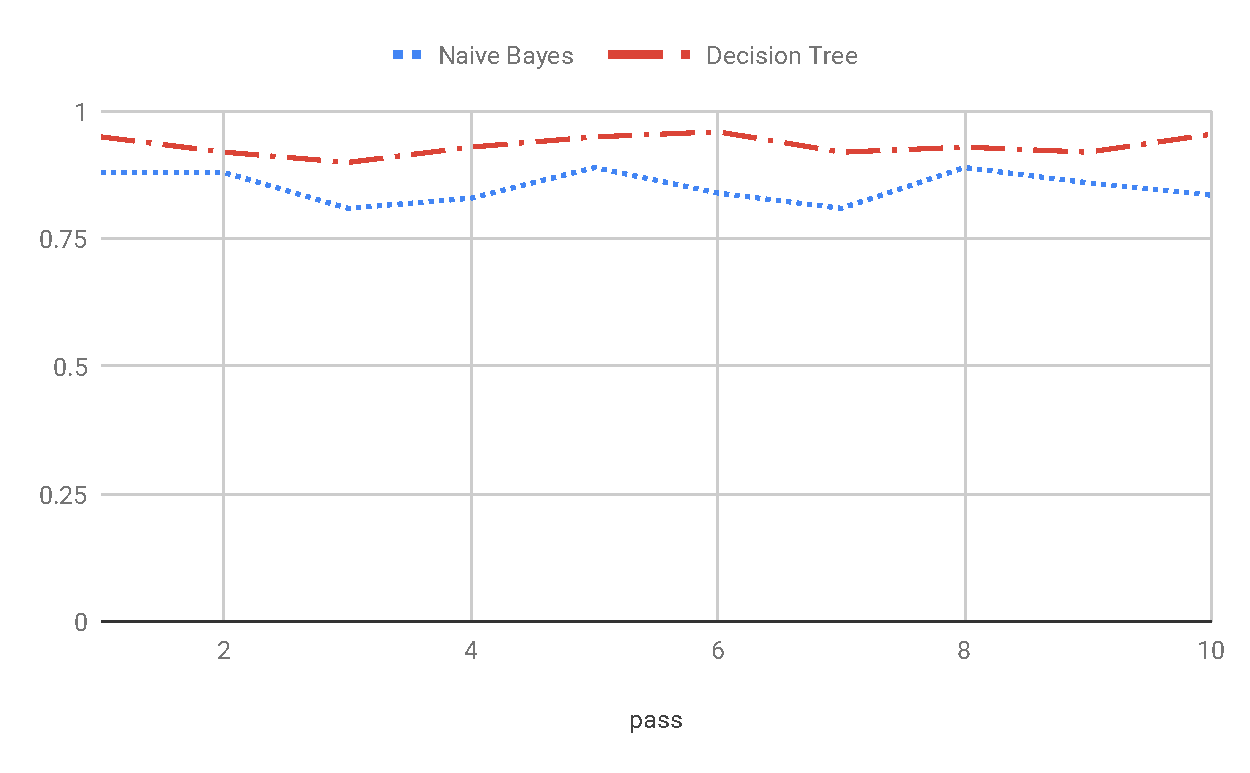
\includegraphics[width=.45\textwidth]{fig/classification.pdf}
	\caption{Accuracy of The 10-fold Validation}
	\label{fig:classification}
\end{figure}
\begin{figure}[hbt]
	\centering
	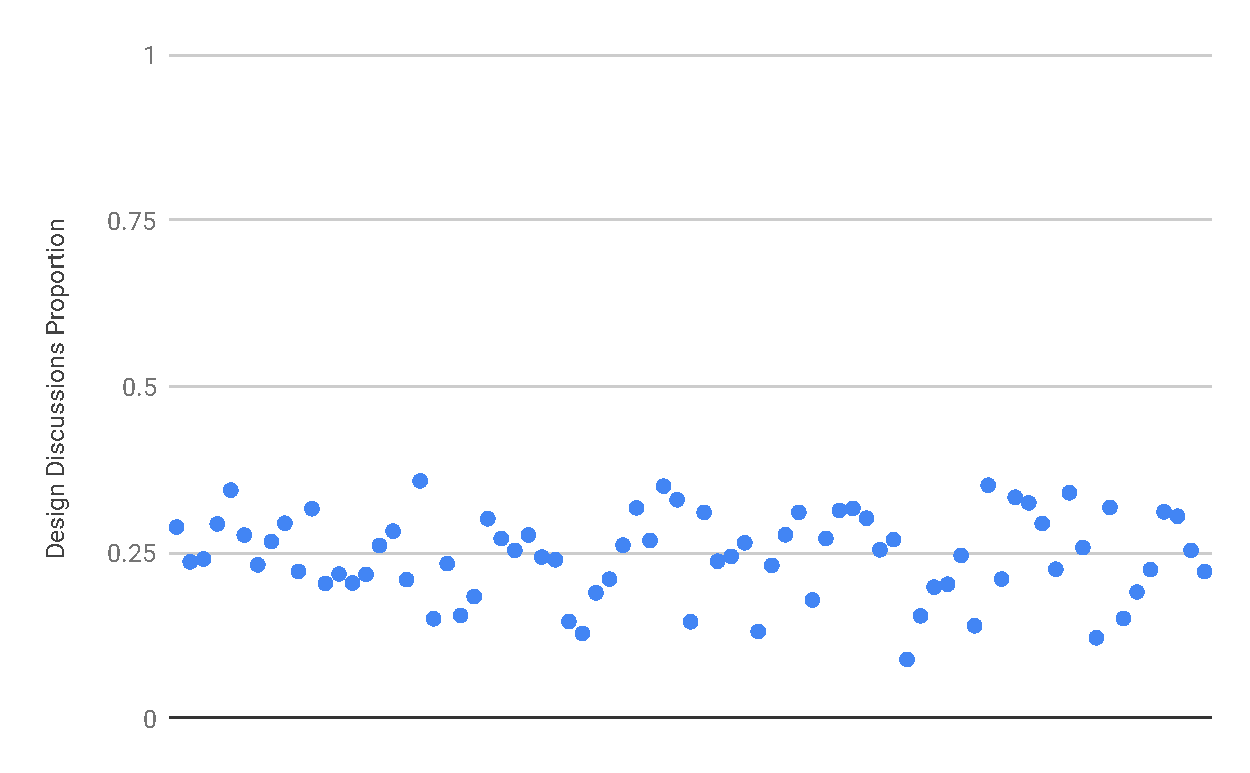
\includegraphics[width=.45\textwidth]{fig/rq_1.pdf}
	\caption{Proportion of Design Discussions Per Project}
	\label{fig:rq_1}
\end{figure}

\begin{figure*}[h!]
	\subcaptionbox{Proportion of Design Discussions Contributors}{%
		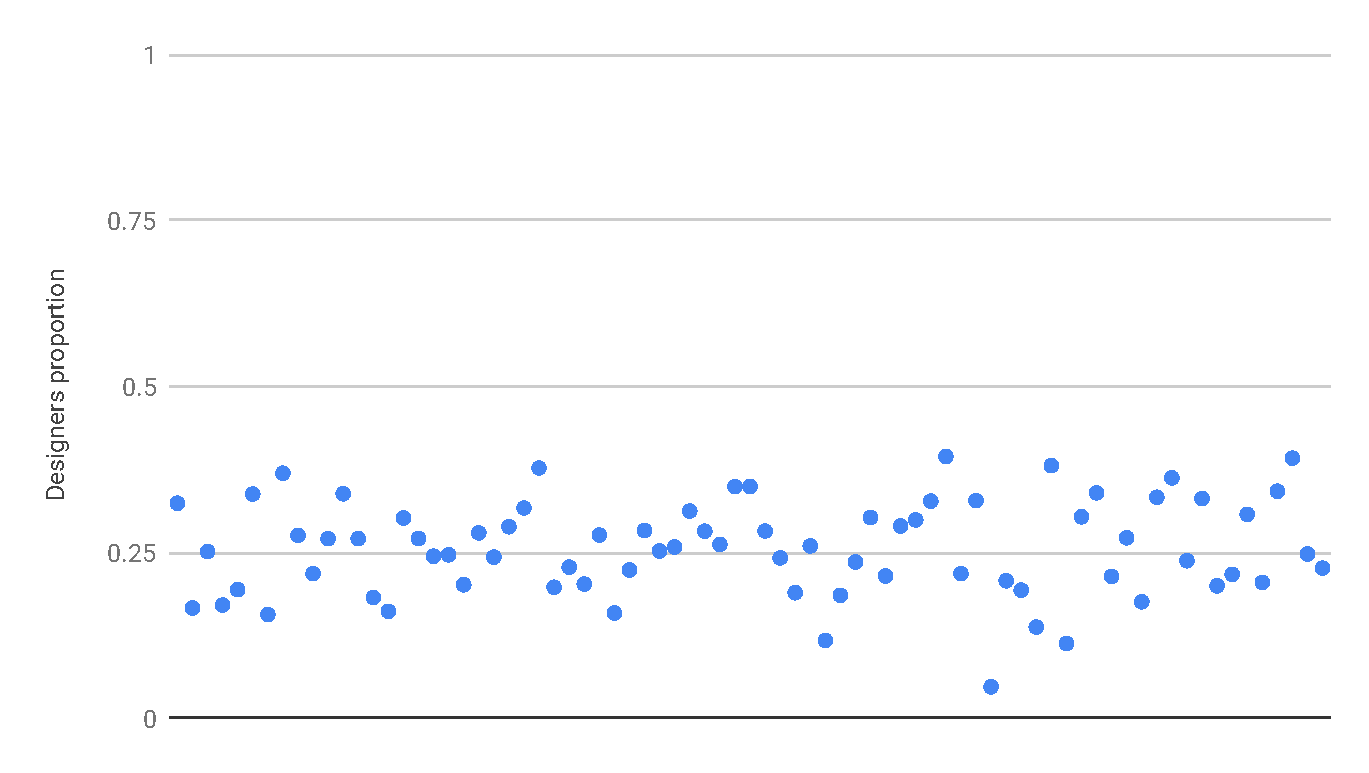
\includegraphics[width=0.30\textwidth]{fig/rq_2_a.pdf}}%
	\hfill
	\subcaptionbox{Developer's Design Discussions Coverage. X-Axis Denotes the Projects and Y-Axis Refers to the Percentage of Coverage}{%
		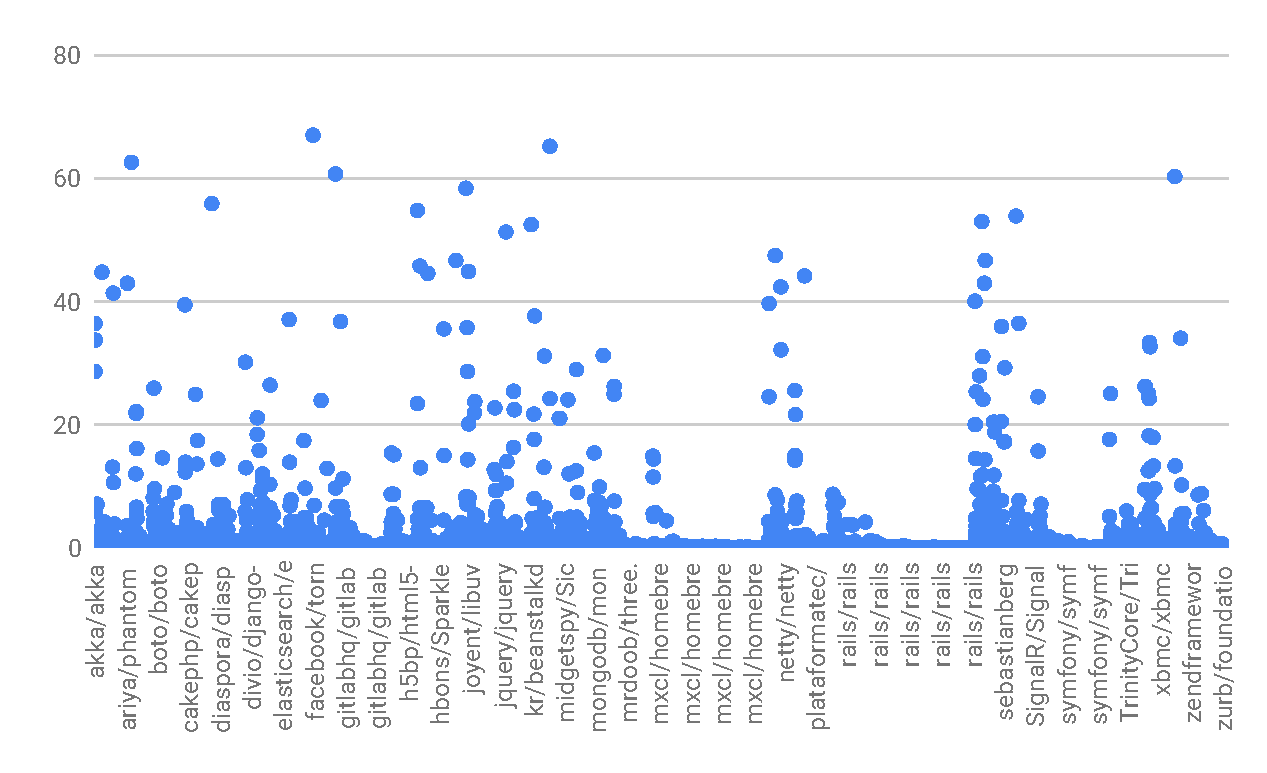
\includegraphics[width=0.30\textwidth]{fig/rq_2_b.pdf}}%
	\hfill
	\subcaptionbox{Developers Coverage with Respect to Commits}{%
		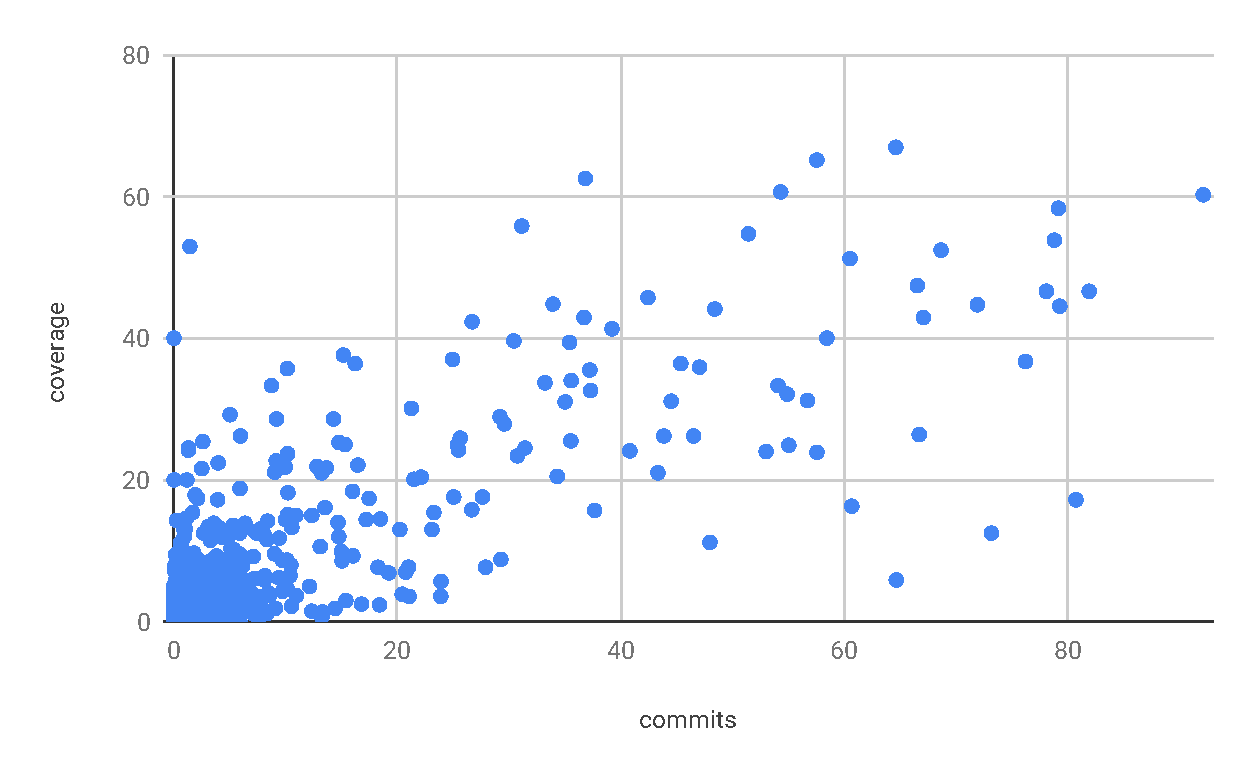
\includegraphics[width=0.30\textwidth]{fig/rq_2_c.pdf}}%
	\caption{Empirical Results}
	\label{fig:rq_2}
\end{figure*}
\section{Results}
\label{sect:results}
After executing the 10-fold cross validation we can see that Decision Tree performs better than Naive Bayes and our result matches the result in~\cite{Brunet2014a}. We achieved 94 {$\pm$} 1\% for Decision Tree and 86 {$\pm$} 1\% for the Naive Bayes classifier which matches with the original paper. The accuracy of each fold of the two classifier can be visualized in Fig. \ref{fig:classification} which clearly shows that Decision Tree outperforms Naive Bayes in every pass. Also as per performance in terms of time, Naive Bayes outperformed Decision Tree by completing almost all the experiments in less than 1 second where Decision Tree took as long as almost 10 minutes in some cases in the same environment.

\subsection{RQ1: To what extent do developers discuss design?}
We have used their processed data to determine the proportion of design discussions for every project. Fig.~\ref{fig:rq_1} shows the proportion of design discussion we can see that, overall 25~{$\pm$}~6\% of the discussions in a project points to some kind of design aspect. We have also observed that our result completely matches with~\cite{Brunet2014a}.

\subsection{RQ2: Which developers discuss design?}
The authors of~\cite{Brunet2014a} analyzed data related to 22,789 developers from the 77 projects that they used. There is no information of how the developers were chosen. So we could not replicate their database pre-processing stage. So, we used their processed data to conduct the empirical study similar to them. After conducting the study, we found very similar results found by them. Similarly, we found that the number of developers involved in design discussions is 8,207 (36\%). Fig.~\ref{fig:rq_2}~(a) shows the proportion of contributors for each project that got involved in design discussions.

In the later experiments, they introduced a term called \emph{Coverage} which indicates the proportion of all design discussions in a project to which a developer has contributed. For example, if a project has 10 design discussions and a developer contributes to 5 of them then the coverage of this developer would be 0.5. In the second step, they found that the majority of developers contributes to less than 10\% of the design discussions. They also found that 99\% of the developers contribute to only 15\% of the design discussions in a specific project. After replicating this, we also have the similar conclusion. Fig.~\ref{fig:rq_2}(b) shows the coverage of developers for a specific project.

The authors in~\cite{Brunet2014a} hypothesized that several factors could be present for developers to contribute to a broad range of design discussions. This scenario implies that these developers have a key role in the projects. They measured the relationship between the proportion of developers commits and their respective coverage. They used Spearman's method which we also used. Eventually we found the same result as they did regarding the relation of developers commits and their coverage. Fig~\ref{fig:rq_2}(c) plots the relation between the percentage of developer commits and their coverage. We found 74\% correlation between those two parameters which is exactly the same as theirs.     
   
% !TEX root = main.tex
\section{Conclusions}
\label{sect:conclusions}
In this work, we tried to replicate the work in~\cite{Brunet2014a} as strictly and identically as possible. In this process, \noindent\textbf{first} we have replicated their steps to build the classifier they used. After building the classifier, we observed that the accuracy they reported exactly matches with the accuracy we obtained. Then in the \noindent\textbf{second} phase, we tried to replicate the empirical study conducted with the classified document. After replicating the study we verified all the results they mentioned in their paper. After doing this study we have come to the conclusion that this study is highly replicable.    


\section*{Acknowledgment}
This work was conducted to fulfill the requirements of graduate assignment of SENG-480 under Professor Neil Ernst. We would like to thank the authors of~\cite{Brunet2014a} in particular Jo\~{a}o Brunet, for providing us with their dataset. 

% TODO balance the columns in the last page (e.g., the bibliography)
% \balance

\bibliographystyle{IEEEtran}
\bibliography{main}

\end{document}
